\section{Forecasting}

In the last part of this project, we want to forecast the monthly mean air temperature in Recife for the year $1996$. We first forecast for the next $12$ months using our SARIMA chosen model.

\begin{figure}[H]
	\centering
	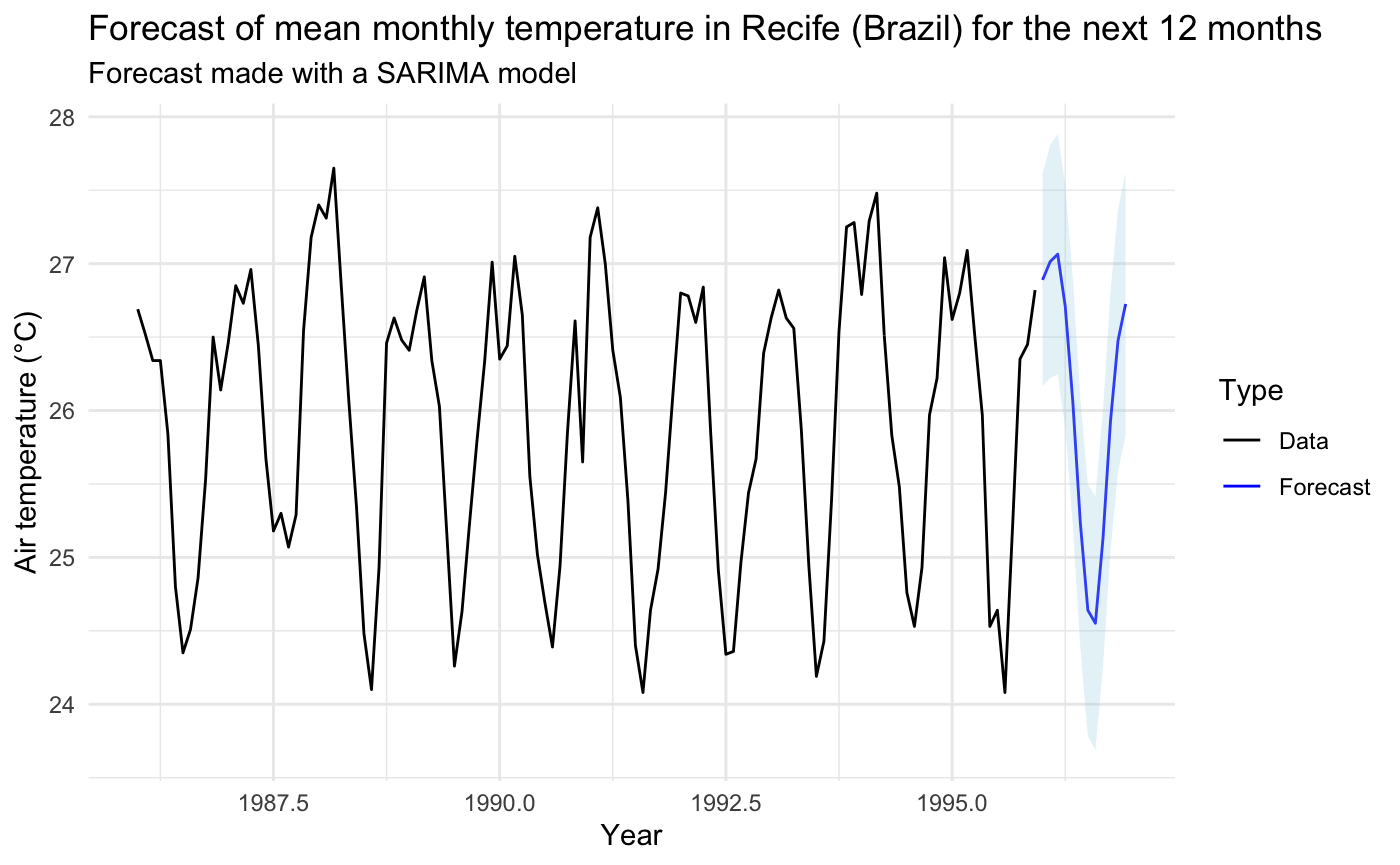
\includegraphics{figures/forecast/sarima_forecast.png}
	\caption{Forecast with a SARIMA model of the mean monthly air temperature in Recife (Brazil) for the next 12 months}
	\label{fig:sarima-forecast}
\end{figure}

Then we would also like to compare this forecast with another one made via the Holt-Winters method.

Holt-Winters' seasonal method is a type of exponential smoothing forecasting method. These methods produce forecasts that consist in weighted averages of past observations where the weights decay exponentially as the observations get older.

Here, we use the Holt-Winters' additive method because our serie shows roughly constant seasonal variations (\autoref{fig:seasonal-plot}). The equation is, 

\begin{equation}
	\hat{X}_{t + H} = l_t + h b_t + s_{t + h - m(k + 1)}
\end{equation}

where $m = 12$ is the number of seasons in a year, $k \equiv int(h - 1) / m$ and $l_t$, $b_t$, and $s_t$ are respectively the smoothing equations for the level $l_t$ of the serie, the trend $b_t$ and the seasonal component $s_t$.

\begin{figure}[H]
	\centering
	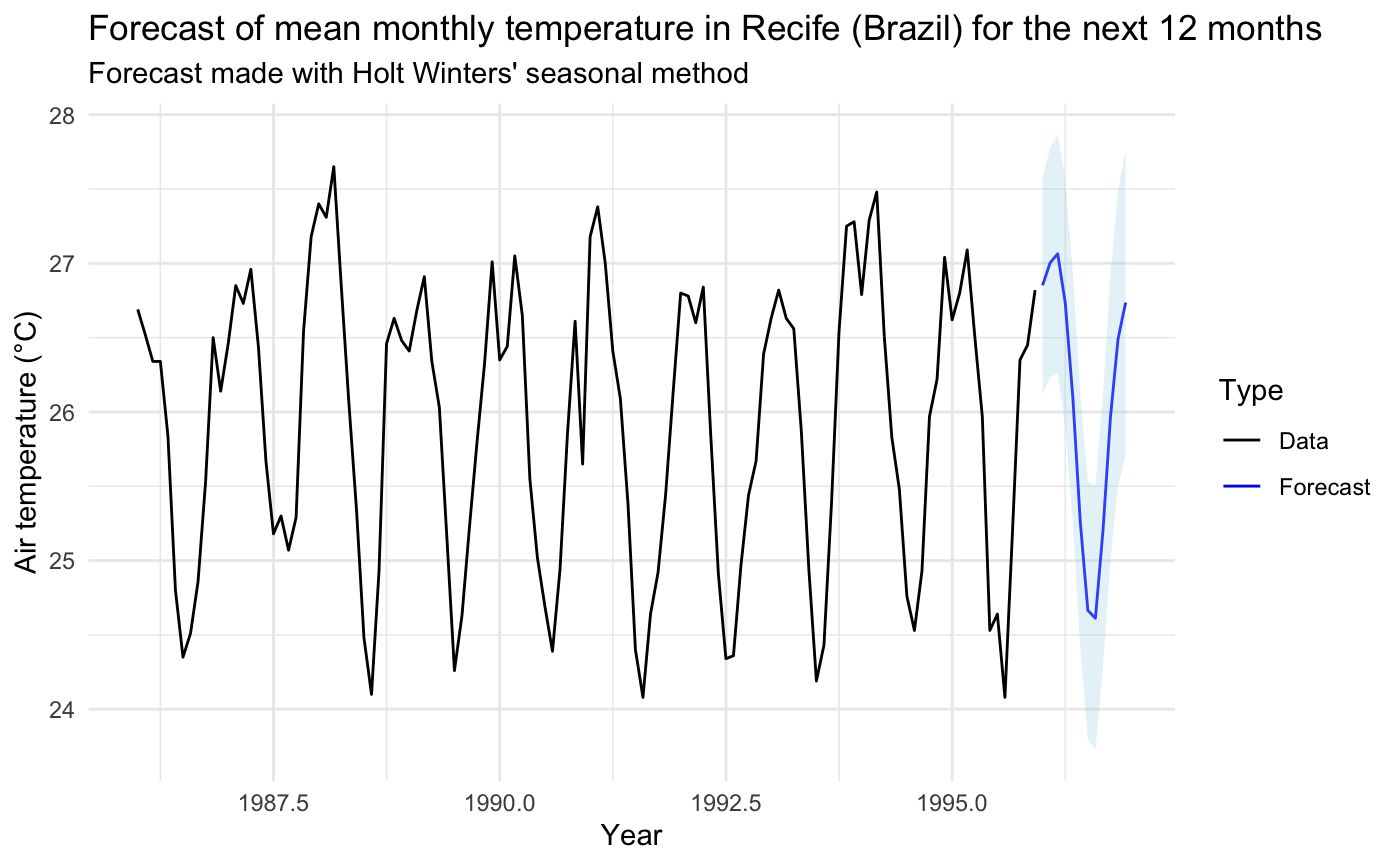
\includegraphics{figures/forecast/hw_forecast.png}
	\caption{Forecast with a Holt-Winters' seasonal method of the mean monthly air temperature in Recife (Brazil) for the next 12 months}
	\label{fig:hw-forecast}
\end{figure}